\section{Architecture}

 \begin{figure}[h]
 \centering
 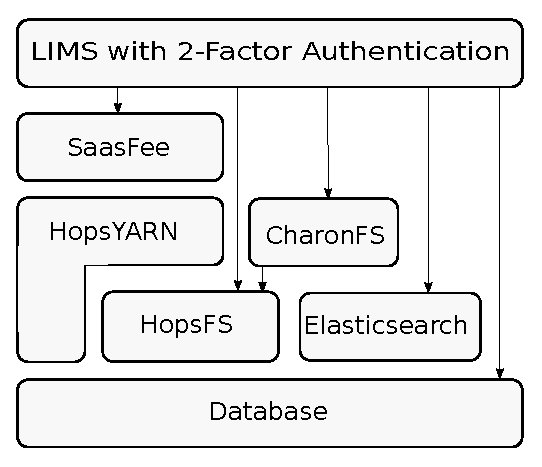
\includegraphics[scale=0.75]{./imgs/stack.eps}
 % stack.eps: 0x0 pixel, 300dpi, 0.00x0.00 cm, bb=0 -1 805 312
 \caption{BiobankCloud Architecture}
 \label{fig:arch}
\end{figure}

Our platform has a layered architecture (see Figure \ref{fig:arch}). In a typical installation, users will access the system through the web interface with 2-factor authentication. From there, she can access all services, such as the enhanced file system HopsFS (see section \ref{hops}), the workflow execution engine SAASFEE (see section \ref{saasfee}), the federated cloud service CharonFS (see section \ref{charonfs}), and an Elasticsearch instance to search through an entire installation. SAASFEE is built over YARN, while CharonFS can use HopsFS as a backing store. HopsFS and  Elasticsearch use a distributed, in-memory database for metadata management. Note that all services can also be accessed directly through command-line interfaces.

\subsection*{Data Sets for Hadoop}

The web interface has integrated a LIMS to manage the typical data items inside a biobank, and to provide fine-grained access control to these items. These items are also reflected in the Hadoop installation. Specifically, 
BiobankCloud introduces \textbf{DataSets} as a new abstraction, where a DataSet consists of a related group of directories, files, and extended metadata. DataSets can be indexed and searched (through Elasticsearch) and are the basic unit of data management in BiobankCloud; all user-generated files or directories belong to a single DataSet. In Biobanking, a sample collection would be a typical example of a DataSet.  To allow for access control of users to DataSets, which is not inherent in the DataSet concept, we introduce the notion of \textbf{Studies}. A Study is a grouping of researchers and DataSets (see Figure \ref{fig:studies}) and the basic unit of privacy protection (see below). 

\begin{figure}[h]
 \centering
 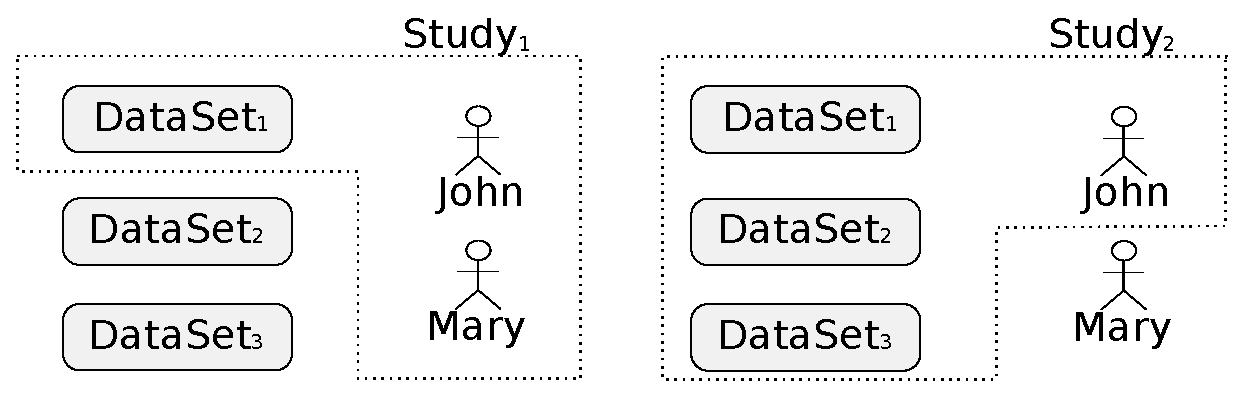
\includegraphics[scale=0.4]{./imgs/projects-as-groupings1.eps}
 % projects-as-groupings1.eps: 0x0 pixel, 300dpi, 0.00x0.00 cm, bb=0 207 582 382.
\caption{Study1 has John and Mary as users and includes DataSet1, while Study2 has only John as as a user and includes DataSet1, DataSet2, and DataSet3.}
\label{fig:studies}
\end{figure}

